\chapter{空白操作系统的启动}

\section{操作系统启动流程}

按下电源键后计算机开始启动,启动过程分为3个阶段\cite{hbt}:
\begin{center}BIOS -> MBR -> 操作系统\end{center}

\begin{enumerate}
\item 在BIOS完成POST(硬件自检,Power-On Self Test)
  并根据启动顺序(Boot Sequence)来选择启动设备。本系统是从U盘启动。
\item 计算机读取该设备的MBR(第一个扇区,最前面的512个字节,见图~\ref{fig:mbr}),
  并运行其中的启动程序IPL(Initial Program Loader),将ZOS加载入内存。本部分的实现
  代码,参见程序~\ref{sec:ipl09.nas};
\item 控制权转交给操作系统后,Kernel开始运行,操作系统启动成功。
\end{enumerate}

\begin{figure}
  \centering
  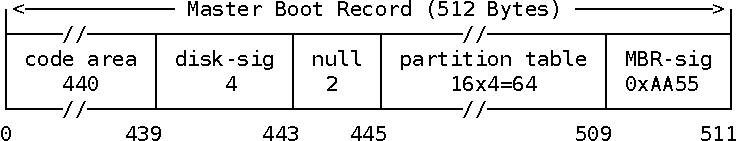
\includegraphics[width=1\textwidth]{fig/mbr.pdf}
  \caption{MBR}
  \label{fig:mbr}
\end{figure}

\section{制作MBR}

MBR负责指出操作系统的位置,主分区第一个扇区的物理位置(柱面、磁头、扇区号等等)

\begin{listing}[H]
  \inputminted[tabsize=2, firstline=6, lastline=6,
  linenos=true]{nasm}{../ZOS/src/kernel/ipl09.nas}
  \inputminted[tabsize=2, firstline=12, lastline=29,
  linenos=true]{nasm}{../ZOS/src/kernel/ipl09.nas}
  \caption{Example of a listing.}
  \label{lst:example}
\end{listing}

\inputminted[tabsize=2, firstline=43, lastline=45,
linenos=true]{nasm}{../ZOS/src/kernel/ipl09.nas}

\inputminted[tabsize=2, firstline=76, lastline=88,
linenos=true]{nasm}{../ZOS/src/kernel/ipl09.nas}

\begin{listing}[H]
  \inputminted[tabsize=2, firstline=125, lastline=147,
  linenos=true]{nasm}{../ZOS/src/kernel/ipl09.nas}
\end{listing}

\section{制作空白操作系统}

为测试操作系统是否成功被MBR启动,设计将操作系统设置为启动后待机。

\begin{minted}[firstnumber=1]{nasm}
    fin:
      HLT
      JMP fin
\end{minted}

按下电源键,经过启动步骤系统循环执行HLT\footnote{HLT: 让CPU停止动作并进入待机状态}使得操作系统计算机始终处于待机状态,启动成功。

